\documentclass[14pt]{extarticle}
\usepackage[T1]{fontenc}
\usepackage[a4paper, total={6in, 8in}]{geometry}
 \geometry{
 a4paper,
 total={170mm,257mm},
 left=29mm,
 top=40mm,
 right=29mm,
 bottom=35mm,
 }
\usepackage{lmodern}

\usepackage{etoolbox}
\usepackage[utf8]{inputenc}
\usepackage[T1]{fontenc}
\usepackage{setspace}
\usepackage{mathptmx}
\usepackage[scaled=.92]{helvet}
\usepackage{charter}
\usepackage[charter]{mathdesign}
\usepackage[scaled]{berasans}
\usepackage{cmbright}
\usepackage[default,scale=0.95]{opensans}
\usepackage[varqu]{zi4}
\usepackage[hyphens]{url}
\usepackage[table]{xcolor}
\usepackage{pgfplots}
\usepackage{newfloat}
\usepackage{tabularx}
\usepackage{xltabular}
\usepackage[USenglish, dutch]{babel}
\usepackage{titlesec}
\usepackage[
    bottom,
    hang,
    multiple
]{footmisc}
\usepackage{chngcntr}
\usepackage{fancyhdr}
\usepackage{parskip}
\usepackage{array}
\usepackage{longtable}
\usepackage{multirow}
\usepackage{adjustbox}
\usepackage{float}
\usepackage{caption}
\usepackage[defaultlines=2,all]{nowidow}
\usepackage[style=english]{csquotes}
\usepackage{enumitem}
\usepackage{footnotebackref}
\usepackage{microtype}


\usepackage{amsmath}
\usepackage{hyperref}
\usepackage{cleveref}
\renewcommand{\familydefault}{\sfdefault}

\usepackage{graphicx} % Required for inserting images
\usepackage{multirow}

\usepackage{siunitx}
\usepackage[american, european resistors, cute inductor, siunitx, nooldvoltagedirection]{circuitikz}

\usetikzlibrary{angles,
                quotes}

\usepackage{tkz-euclide}

\usepackage{mathtools}

\title{Aantekeningen eps20}
\author{Jasmine Hottentot}
\date{December 2025}

\begin{document}
\maketitle
\newpage
\tableofcontents
\newpage
\section{Vermogen en blind vermogen}
\input{vermogen berekenen.tex}
\subsection{Impendantie driehoek}
Voor de impendantie is ook een driehoek te maken. Dit is de driehoek voor een spoel.

\begin{center}

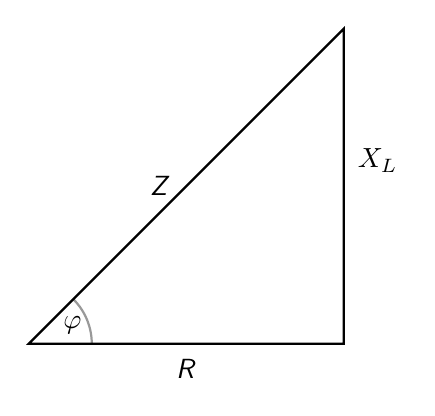
\begin{tikzpicture}[thick]
\coordinate (O) at (0,0);
\coordinate (A) at (4,0);
\coordinate (B) at (4,4);
\draw (O)--(A)--(B)--cycle;

\tkzLabelSegment[below=2pt](O,A){\textit{R}}
\tkzLabelSegment[left=2pt](O,B){\textit{Z}}
\tkzLabelSegment[above right=2pt](A,B){\textit{$X_L$}}

\tkzMarkAngle[fill= teal,size=0.8cm,%
opacity=.4](A,O,B)
\tkzLabelAngle[pos = 0.6](A,O,B){$\varphi $}

\end{tikzpicture}
\end{center}

Hier geldt:\\
R= weerstand\\
Z= impendantie\\
$X_L$= inductieve reactantie\\

De verschillen de waardes kunnen bepaald worden op de zelfde manier als bij de vermogensdriehoek.

\vspace{5mm}

Voor de Condensator geld het zelfde alleen is $X_L$ vervangen door $X_C$ en is de impendantie negatief.

\begin{center}

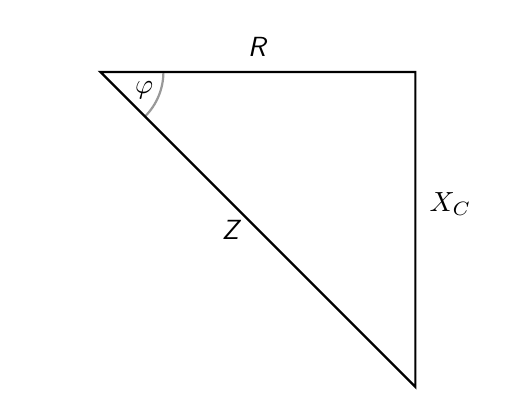
\begin{tikzpicture}[thick]
\coordinate (O) at (0,0);
\coordinate (A) at (4,0);
\coordinate (B) at (4,-4);
\draw (O)--(A)--(B)--cycle;

\tkzLabelSegment[above=2pt](O,A){\textit{R}}
\tkzLabelSegment[left=2pt](O,B){\textit{Z}}
\tkzLabelSegment[above right=2pt](A,B){\textit{$X_C$}}

\tkzMarkAngle[fill= teal,size=0.8cm,%
opacity=.4](B,O,A)
\tkzLabelAngle[pos = -0.6](A,O,B){$\varphi $}

\end{tikzpicture}
\end{center}
\section{Transformatoren}
Het schema voor de transformer kan op de volgende manier worden getekend:

\begin{center}
    \begin{circuitikz} 
        \draw (-1,-2) to[isourcesin] (-1,2);
        \draw (-1,2) to[short] (2,2);
        \draw (2,2) to[short] (2,1);
        \draw (3,1) to[short] (1,1);
        \draw (1,1) to[cute inductor, l_=$jX_c$, i_=$I_0$] (1,-1);
        \draw (3,1) to[american resistor, l_=$R_c$] (3,-1);
        \draw (3,-1) to[short] (1,-1);
        \draw (2,-1) to[short] (2,-2);
        \draw (2,-2) to[short] (-1,-2);
        \draw (2,2) to[short] (4,2);
        \draw (4,2) to[L, l=$jX_1$, i_=$I_1$] (6,2);
        \draw (6,2) to[american resistor, l_=$R_1$] (9,2);
        \draw (9,2) to[cute inductor] (9,-2);
        \draw (9,-2) to[short] (2,-2);
        \draw (10,2) to[cute inductor] (10,-2);
        \draw (10,2) to[L, l=$jX_2$, i_=$I_2$] (12,2);
        \draw (12,2) to[american resistor, l_=$R_2$] (14,2);
        \draw (14,2) to[european resistor, l_=$R_L$] (14,-2);
        \draw (14,-2) to[short] (10,-2);
        \draw (8,2) to [open, v^>=$V_1$] (8,-2);
        \draw (11,2) to [open, v^>=$V_2$] (11,-2);
    \end{circuitikz}
\end{center}

\end{document}